\chapter{Risultati sperimentali} % (fold)
\label{chap:Risultati sperimentali}

\section{Addestramento} % (fold)
\label{sec:Addestramento}

Il modello \`e stato addestrato mediante l'uso della \textit{cross-validation}(\autoref{fig:cross_validation})
con una suddivisione dei dati in cinque parti uguali(cinque folds).

Essendo una tipologia di apprendimento supervisionata, al modello sono fornite immagini
originali e le loro segmentazioni effettuate manualmente.

\begin{figure}[!ht]
    \centering
    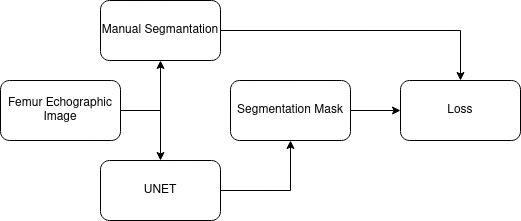
\includegraphics[width=0.7\columnwidth]{Immagini/training.png}
    \caption{Addestramento del modello}
    \label{fig:addestramento del modello}
\end{figure}


Effettuando l'addestramento con 5 folds, il modello viene addestrato 5 volte, ogni volta con un fold diverso,
l'errore finale \`e dato dalla media degli errori ottenuti dalle 5 iterazioni.

\begin{figure}[!ht]
    \centering
    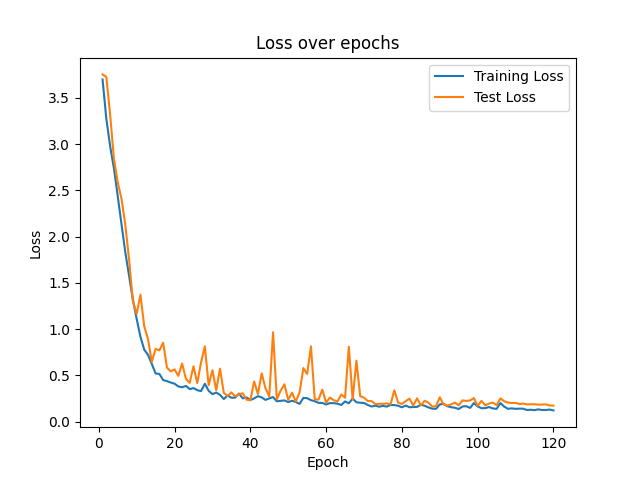
\includegraphics[width=0.4\columnwidth]{Immagini/fold_0_loss.png} 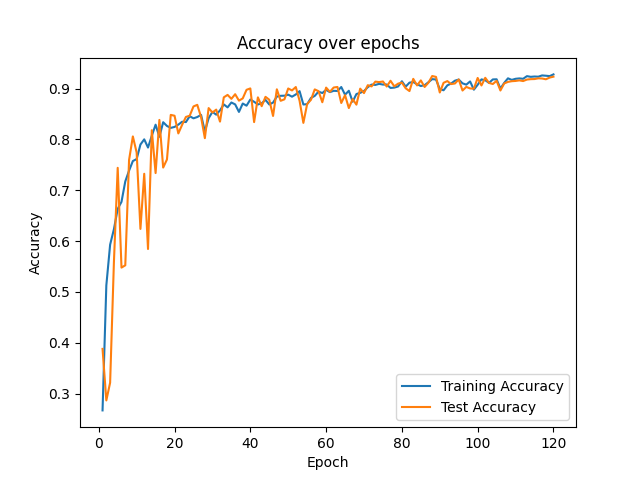
\includegraphics[width=0.4\columnwidth]{Immagini/fold_0_accuracy.png}
    \caption{Errore e accuratezza della prima porzione di dati}
    \label{fig:loss e accuratezza della prima porzione di dati}
\end{figure}

\begin{figure}
    \centering
    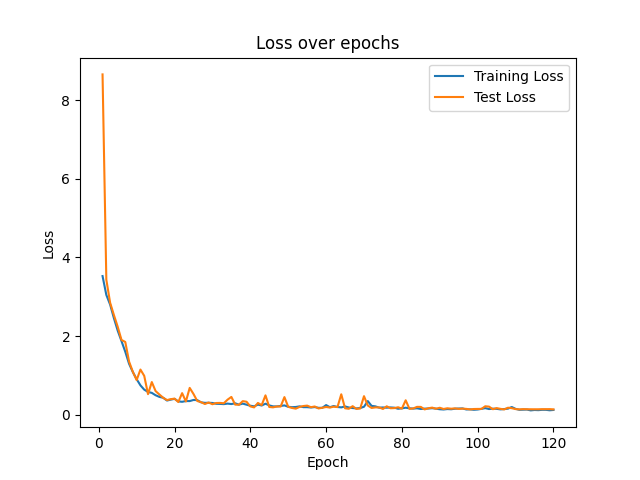
\includegraphics[width=0.4\columnwidth]{Immagini/fold_1_loss.png} 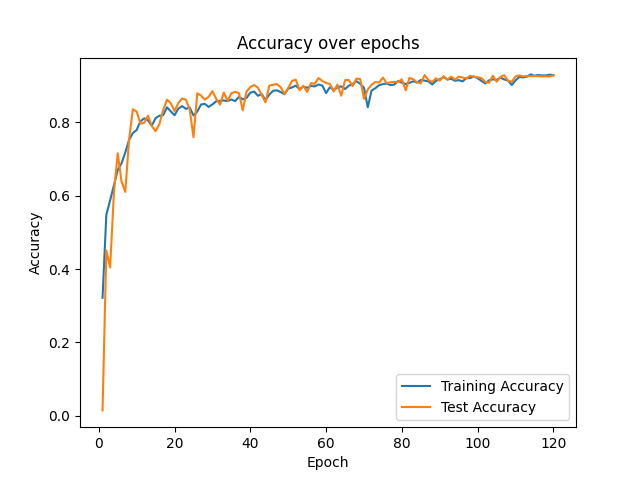
\includegraphics[width=0.4\columnwidth]{Immagini/fold_1_accuracy.png}
    \caption{Errore e accuratezza della seconda porzione di dati}
    \label{fig:loss e accuratezza della seconda porzione di dati}
\end{figure}

\begin{figure}
    \centering
    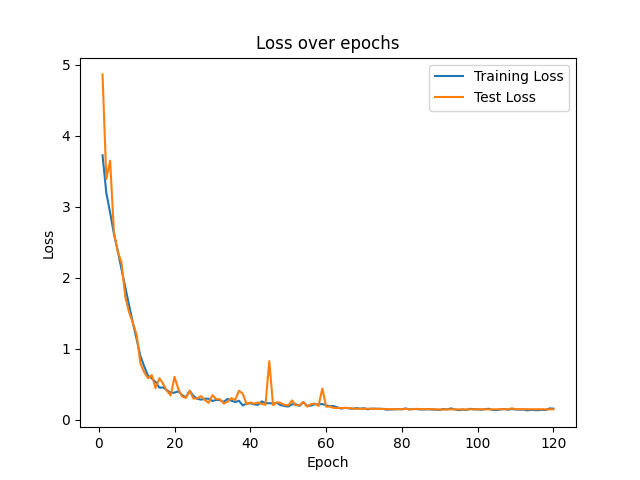
\includegraphics[width=0.4\columnwidth]{Immagini/fold_2_loss.png} 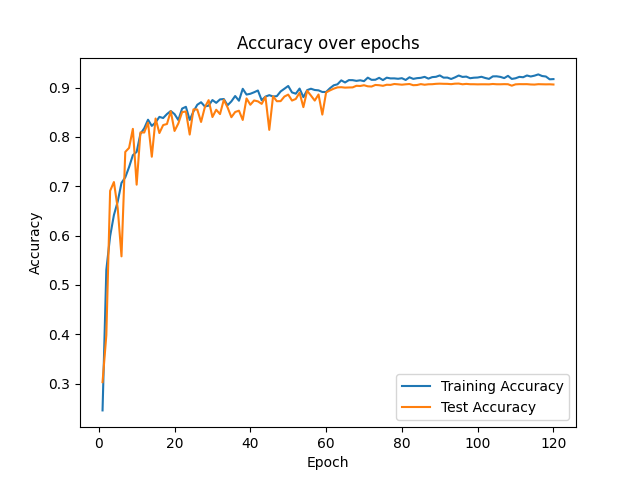
\includegraphics[width=0.4\columnwidth]{Immagini/fold_2_accuracy.png}
    \caption{Errore e accuratezza della terza porzione di dati}
    \label{fig:loss e accuratezza della terza porzione di dati}
\end{figure}

\begin{figure}
    \centering
    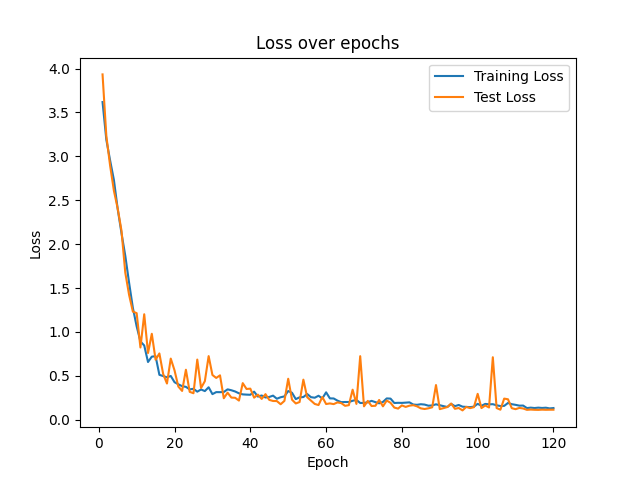
\includegraphics[width=0.4\columnwidth]{Immagini/fold_3_loss.png} 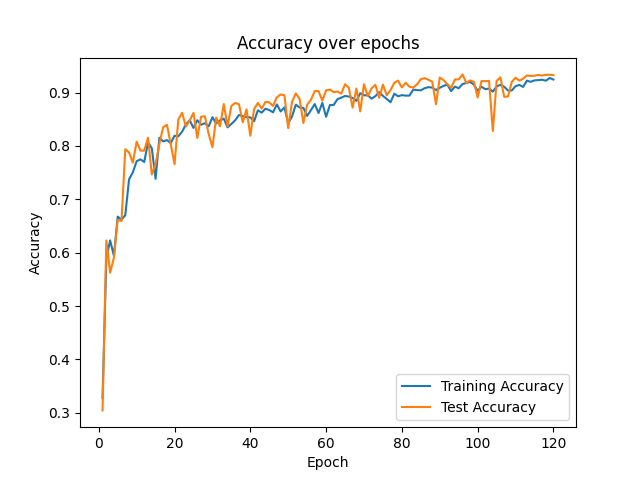
\includegraphics[width=0.4\columnwidth]{Immagini/fold_3_accuracy.png}
    \caption{Errore e accuratezza della quarta porzione di dati}
    \label{fig:loss e accuratezza della quarta porzione di dati}
\end{figure}

\begin{figure}
    \centering
    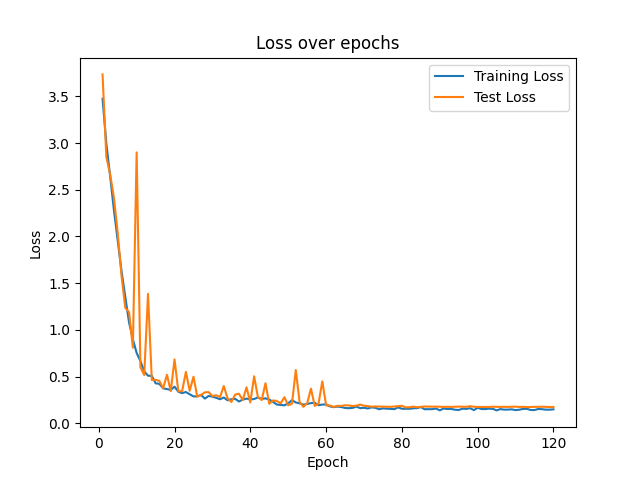
\includegraphics[width=0.4\columnwidth]{Immagini/fold_4_loss.png} 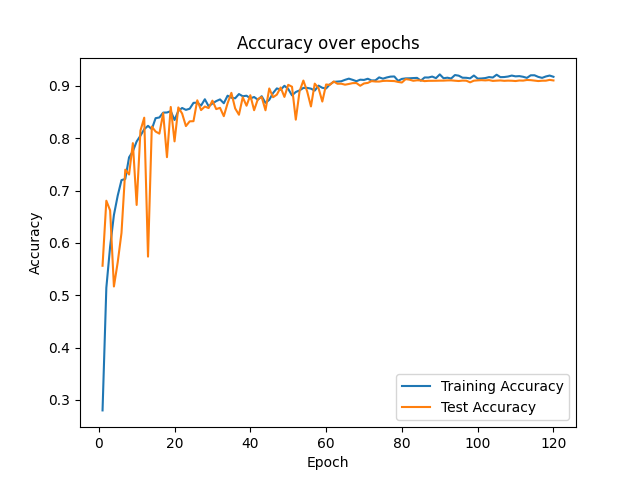
\includegraphics[width=0.4\columnwidth]{Immagini/fold_4_accuracy.png}
    \caption{Errore e accuratezza della quinta porzione di dati}
    \label{fig:loss e accuratezza della quinta porzione di dati}
\end{figure}

L'\textbf{errore} complessivo viene calcolato come media dei singoli errori
ottenuti dalle cinque iterazioni mediante la formula
\ref{eq:dice_bce_loss_complete} portando a un errore medio del
\textbf{$7.9\%$}.

Mentre l'\textbf{accuratezza} complessiva viene calcolata come media delle singole accuratezze
ottenute dalle cinque iterazioni mediante la formula \ref{eq:iou} portando a un'accuratezza media del \textbf{$92.1\%$}.




Considerando che questo modello \`e stato utilizzato in ambito medico per velocizzare e standardizzare 
la segmentazione dei femori per un'analisi su questi ultimi, oltre ad analisi quantitative, \`e stato 
necessario effettuare delle analisi qualitative sulla segmentazione ottenuta dal modello.

Nelle immagini seguenti viene riportato uno delle immagini prese in considerazione per l'addestramento del modello
e vengono mostrate le segmentazione manuali, le segmentazioni ottenute dal modello e la differenze 
nella classificazione dei pixel tra le due segmentazioni.





Partendo da una immagini (\autoref{fig:immagine originale}) ottenuta mediante la raccolta dati effettuata dai medici, 

\begin{figure}[!ht]
    \centering
    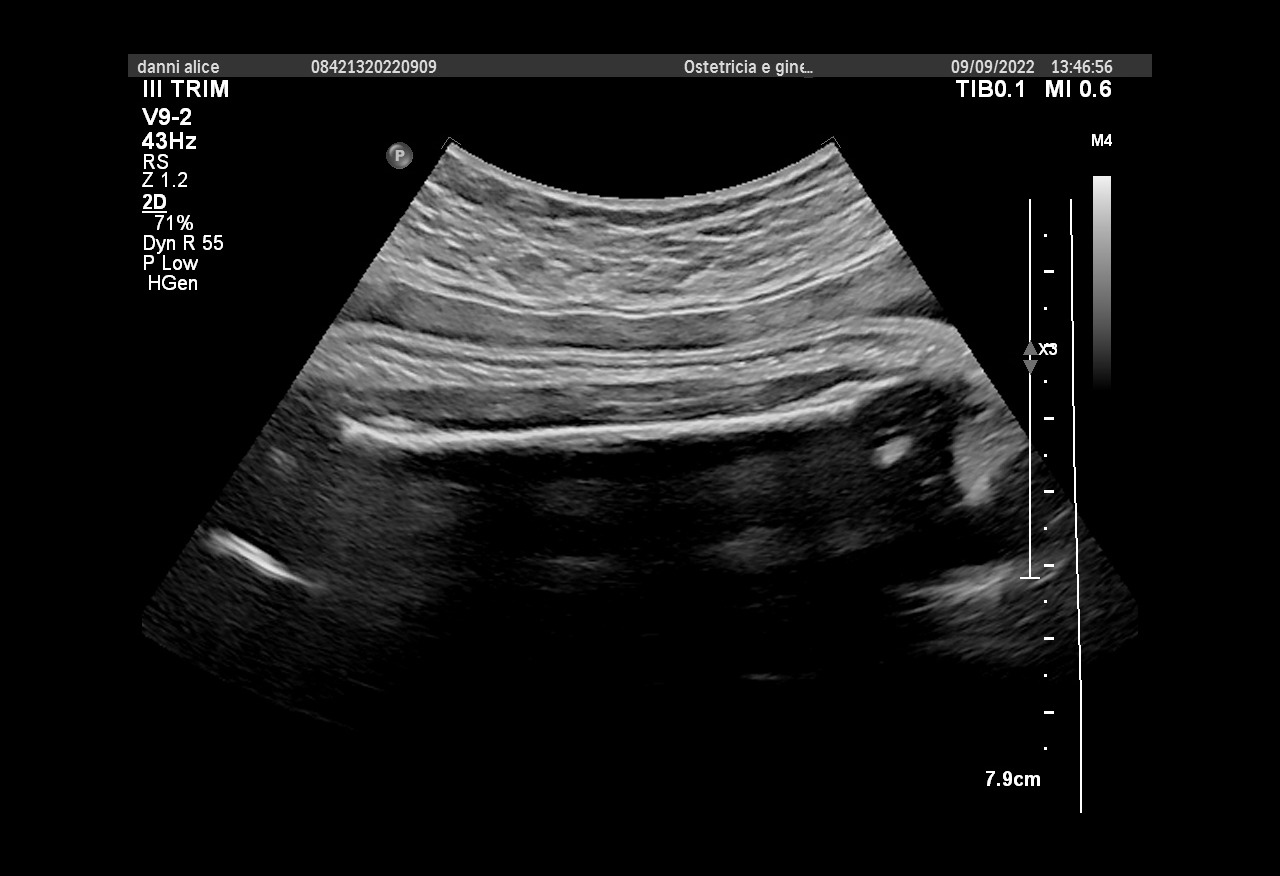
\includegraphics[width=0.7\columnwidth]{Immagini/image.png}
    \caption{Immagine originale}
    \label{fig:immagine originale}
\end{figure}


% I risultati ottenuti mediante la segmentazione manuale e la segmentazione del modello sono 
% rispettivamente \autoref{fig:segmentazione manuale} e \autoref{fig:segmentazione del modello}.

% \begin{figure}[!ht]
%     \centering
%     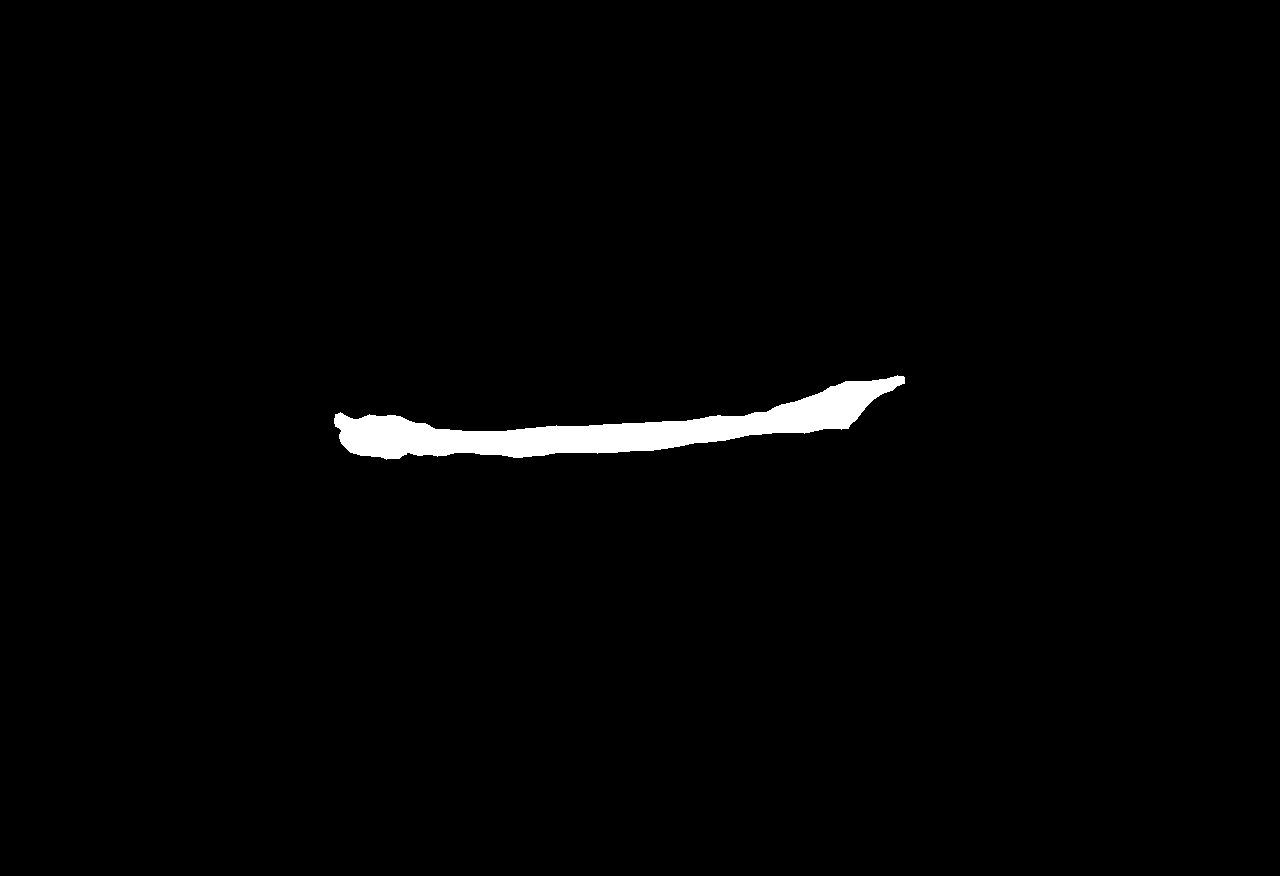
\includegraphics[width=0.4\columnwidth]{Immagini/mask.png}
%     \caption{Segmentazione manuale}
%     \label{fig:segmentazione manuale}
% \end{figure}

% \begin{figure}[!ht]
%     \centering
%     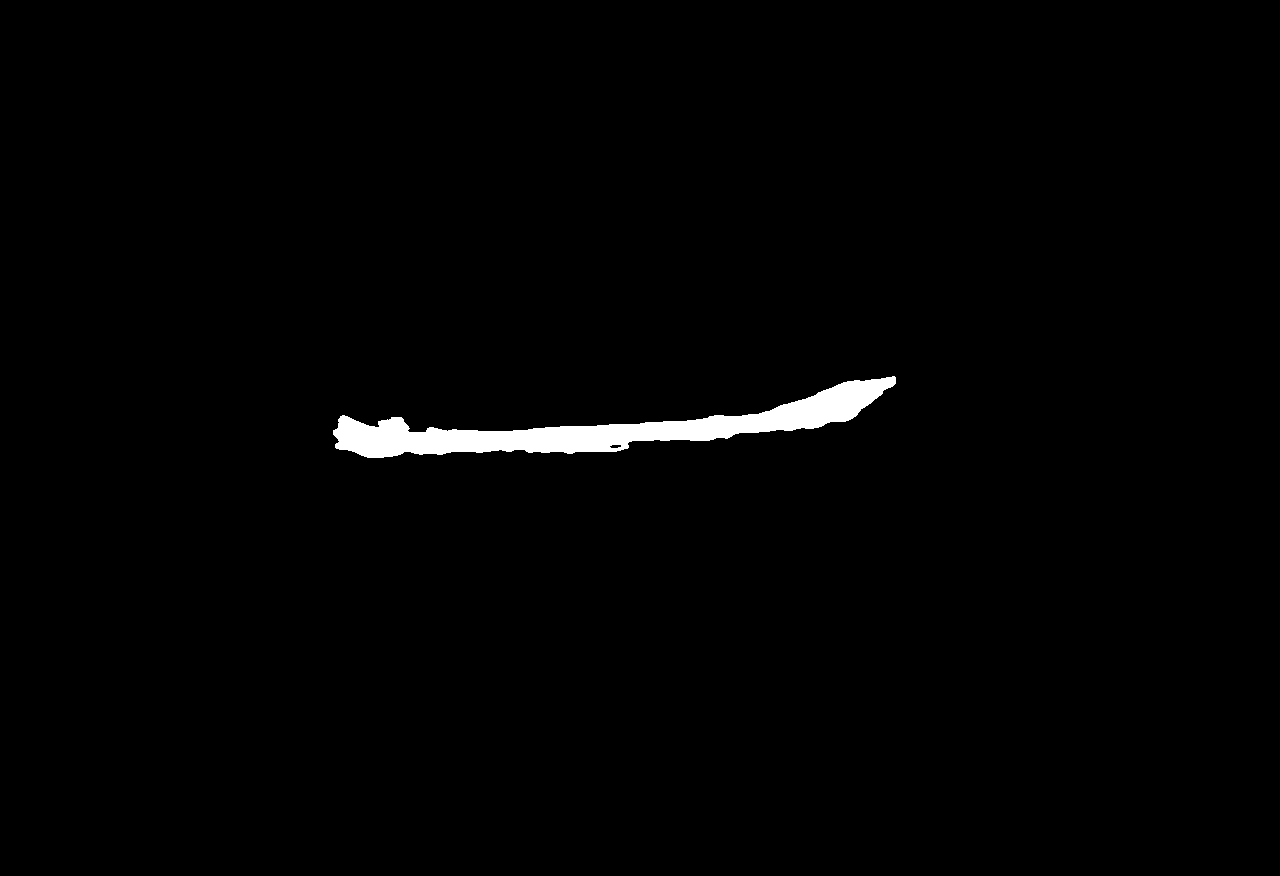
\includegraphics[width=0.4\columnwidth]{Immagini/prediction.png}
%     \caption{Segmentazione del modello}
%     \label{fig:segmentazione del modello}
% \end{figure}

\begin{figure}[!ht]
    \centering
    \begin{minipage}{0.4\columnwidth}
        \centering
        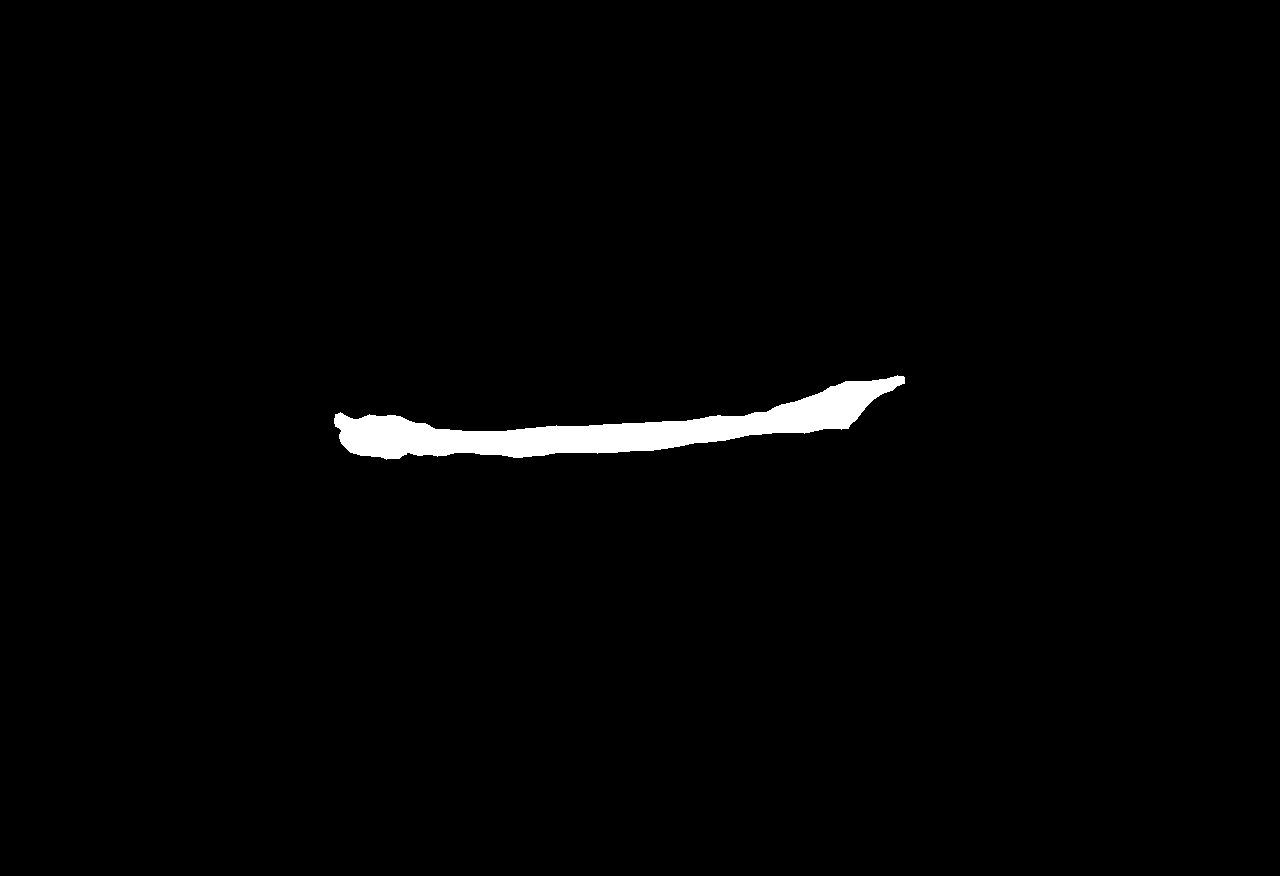
\includegraphics[width=\linewidth]{Immagini/mask.png}
        \caption{Segmentazione manuale}
        \label{fig:segmentazione manuale}
    \end{minipage}
    \hfill
    \begin{minipage}{0.4\columnwidth}
        \centering
        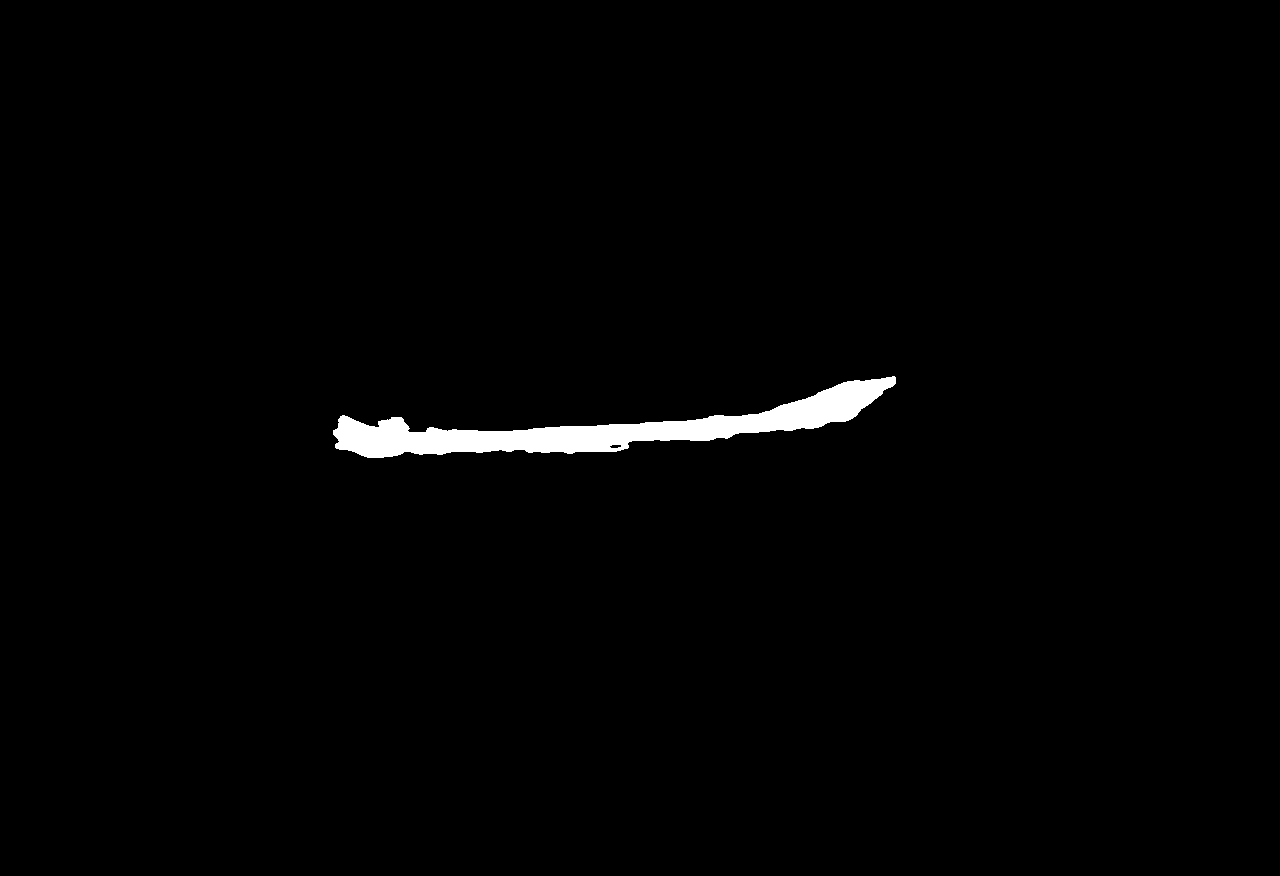
\includegraphics[width=\linewidth]{Immagini/prediction.png}
        \caption{Segmentazione del modello}
        \label{fig:segmentazione del modello}
    \end{minipage}
\end{figure}

Per sostenere la tesi che il modello riesca a segmentare correttamente le immagini, \`e stata 
calcolata la distribuzione dei pixel per confrontare la segmentazione manuale con quella del modello.

% Per quantifica la differenza tra le due segmentazioni \`e stata calcolata la distribuzione dei pixel
% nelle immagini processate manuale e si \`e confrontata con la distribuzione dei pixel nelle immagini
% processate dal modello

% \begin{figure}[!ht]
%     \centering
%     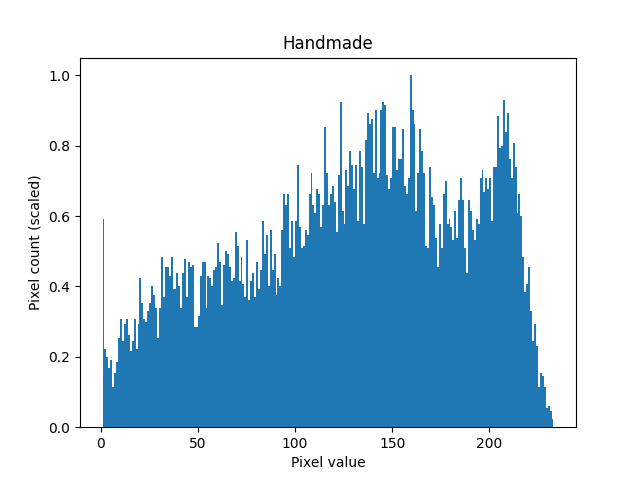
\includegraphics[width=0.7\columnwidth]{Immagini/handmade_scaled_hist.png}
%     \caption{Distribuzione Intensità dei pixel della segmentazione manuale}
%     \label{fig:distribuzione intensità dei pixel della segmentazione manuale}
% \end{figure}

% \begin{figure}[!ht]
%     \centering
%     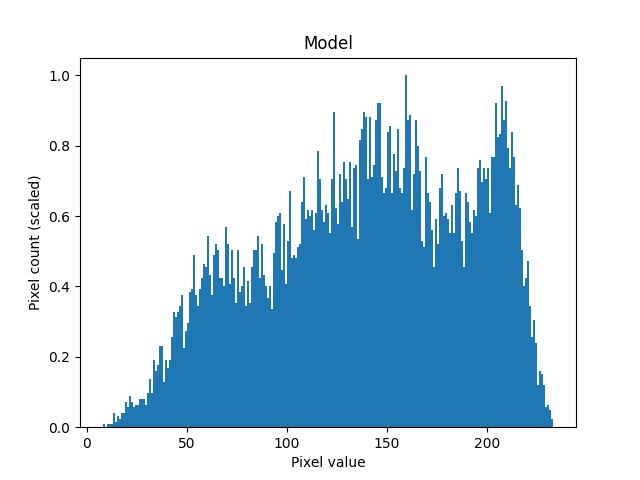
\includegraphics[width=0.7\columnwidth]{Immagini/model_scaled_hist.png}
%     \caption{Distribuzione Intensità dei pixel della segmentazione del modello}
%     \label{fig:distribuzione intensità dei pixel della segmentazione del modello}
% \end{figure}

\begin{figure}[!ht]
    \centering
    \begin{minipage}{0.45\columnwidth}
        \centering
        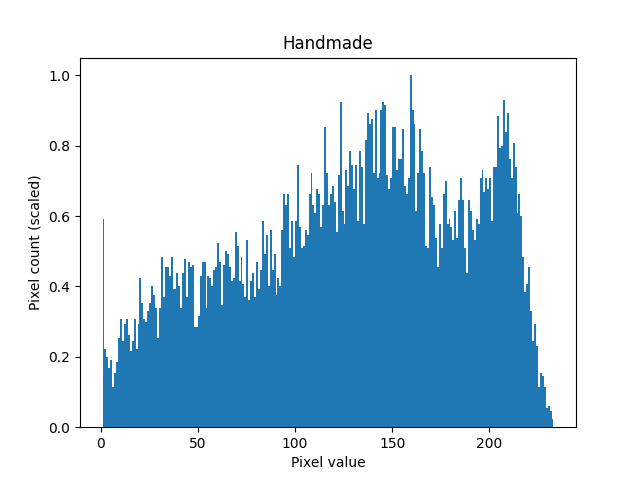
\includegraphics[width=\linewidth]{Immagini/handmade_scaled_hist.png}
        \caption{Distribuzione Intensità dei pixel della segmentazione manuale}
        \label{fig:distribuzione intensità dei pixel della segmentazione manuale}
    \end{minipage}
    \hfill
    \begin{minipage}{0.45\columnwidth}
        \centering
        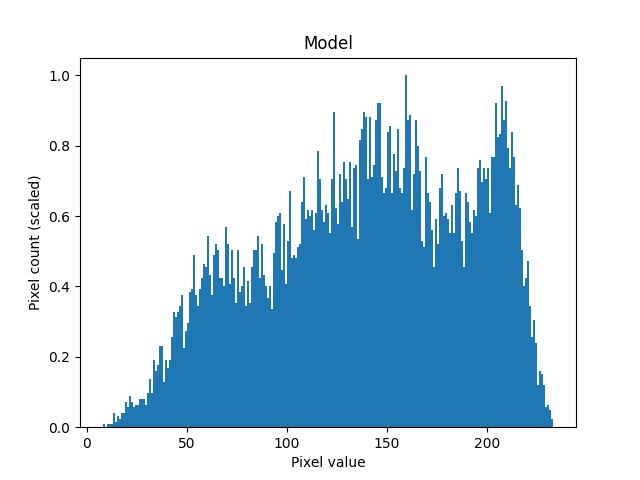
\includegraphics[width=\linewidth]{Immagini/model_scaled_hist.png}
        \caption{Distribuzione Intensità dei pixel della segmentazione del modello}
        \label{fig:distribuzione intensità dei pixel della segmentazione del modello}
    \end{minipage}
\end{figure}

\begin{figure}[!ht]
    \centering
    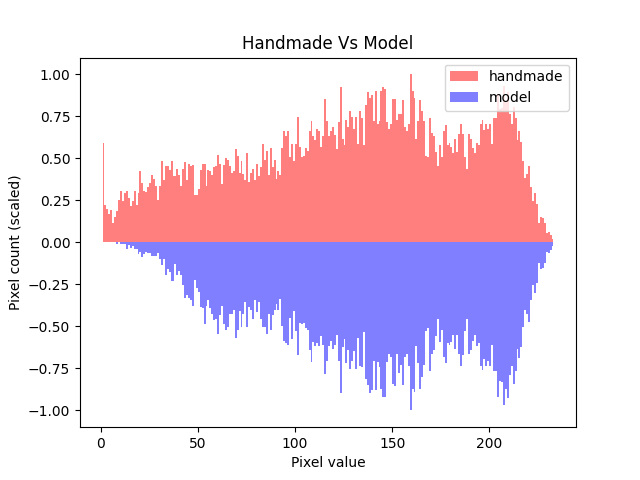
\includegraphics[width=0.7\columnwidth]{Immagini/handmade_vs_model_scaled.png}
    \caption{Confronto tra la segmentazione manuale e quella del modello}
    \label{fig:confronto tra la segmentazione manuale e quella del modello}
\end{figure}


Dai risultati qualitativi e quantitativi si pu\`o constatare che il modello ha una performance
molto promettente in quanto supera abbondantemente un'accuratezza del $90\%$ e pu\`o essere 
addestrato incrementando il numero d'immagini a disposizione. 

Non sono necessari ulteriori segmentazioni manuali ma si possono direttamente sfruttare
le nuove immagini raccolte, segmentarle mediante l'uso del modello e utilizzarle per l'addestramento.




% % section Addestramento (end)





% % chapter Risultati sperimentali (end)
